\section{Model Details}\label{app.model}
Table~\ref{tab:notation} summarizes the notation used.
\begin{table}[h]
  \centering
  \caption{Notation}
  \label{tab:notation}
  \begin{tabular}{cl}
  \toprule
     Symbol     & Definition                                                \\
  \midrule
       $c$      & city index $\in$\{A, B\}                                  \\
       $r$      & risk group index $\in$ \{high, low\}                      \\
       $y$      & type of contact index $\in$ \{sexual, close non-sexual\}  \\
       $x'$     & index ``$x$'' for a contact, versus self                  \\[1ex]
       $N$      & population size                                           \\
       $C$      & contact rate                                              \\
       $Q$      & total contacts offered: $NC$                              \\
   $\epsilon$   & assortativity parameter $\in$ [1: assortative, 0: random] \\[1ex]
    $\lambda$   & incidence rate (force of infection)                       \\
     $\beta$    & secondary attack rate\tn{a}                               \\
  $\sigma^{-1}$ & duration of latent/incubation period                      \\
  $\gamma^{-1}$ & duration of infectious/symptom period                     \\
     $\Phi$     & probability of contact formation                          \\[1ex]
     $\rho$     & proportion isolating among infectious                     \\
      $\nu$     & vaccination rate                                          \\
       $f$      & vaccine effectiveness (leaky-type)                        \\
  \bottomrule
\end{tabular}
\floatfoot
All durations in days; all rates in per-day.
\tnt[a]{per-partnership transmission probability.}
\end{table}
\subsection{Differential Equations}\label{app.model.eqn}
Equation~\eqref{eq:ode} summarizes the system of differential equations for the SVEIR health states;
each equation is repeated for each combination of city~$c$ (A,~B) and risk group~$r$ (high,~low) (4 total),
but we omit the $cr$ index notation for clarity.
\begin{subequations}\label{eq:ode}
  \begin{alignat}{5}
    \frac{d}{dt}&S   &&= - \nu S - \lambda S \\
    \frac{d}{dt}&V   &&= + \nu S - (1 - f) \lambda V \\
    \frac{d}{dt}&E   &&= + \lambda S + (1-f) \lambda V - \sigma E\\
    \frac{d}{dt}&\,I &&= + \sigma E - \gamma I \\
    \frac{d}{dt}&R   &&= + \gamma I
  \end{alignat}
\end{subequations}
\subsection{Incidence Rate}\label{app.model.inc}
The incidence rate (force of infection) for
non-vaccinated susceptible individuals in city $c$ and risk group $r$ (``group $cr$'') is defined as:
\begin{equation}
  \lambda_{cr} = \sum_{yc'r'} (1 - \rho)\,\beta_{y}\,C_{ycr}\,\Phi_{ycrc'r'} \frac{I_{c'r'}}{N_{c'r'}}
\end{equation}
where:
$\rho$ is the proportion isolating among infectious;
$\beta_{y}$ is the transmission probability per type-$y$ contact;
$C_{ycr}$ is the type-$y$ contact rate among group $cr$;
$\Phi_{ycrc'r'}$ is the probability of type-$y$ contact formation with group $c'r'$ among group $cr$; and
$N_{cr}$ is the size of group $cr$.
\par
Among vaccinated, the incidence rate is simply reduced by a factor $(1-f)$, where
$f$ is the vaccine effectiveness (leaky-type).
\subsection{Mixing}\label{app.model.mix}
Mixing between risk groups and cities was implemented using
an adaptation of a common approach \cite{Nold1980,Garnett1994}.
We denote the total contacts ``offered'' by group~$cr$ as: $Q_{cr} = N_{cr} C_{cr}$;
and denote the margins $Q_{c} = \sum_{r}Q_{cr}$; $Q_{r} = \sum_{c} Q_{cr}$; and $Q = \sum_{cr}Q_{cr}$.
The probability of contact formation with group $c'r'$ among group $cr$ is defined as:
\begin{equation}
  \Phi_{crc'r'} =
    \epsilon_c \delta_{cc'} \left(
      \epsilon_r \delta_{rr'} + (1 - \epsilon_r) \frac{Q_{c'r'}}{Q_{c'}}
    \right) +
    (1 - \epsilon_{c}) \frac{Q_{c'}}{Q} \left(
      \epsilon_r \delta_{rr'} + (1 - \epsilon_r) \frac{Q_{r'}}{Q}
    \right)
\end{equation}
where:
$\delta_{ii'} = \{1~\text{if}~i = i'; 0~\text{if}~i \ne i'\}$ is an identity matrix; and
$\epsilon_{c}, \epsilon_{r} \in [0,1]$ are assortativity parameters
for mixing among cities and risk groups, respectively, such that
$\epsilon = 1$ yields complete group separation and
$\epsilon = 0$ yields completely random (proportionate) mixing.
For clarity, we omit the index of contact type $y$,
although $\epsilon_r$, $C_{cr}$ and thus $\Phi_{crc'r'}$ are all further stratified by $y$.
\subsection{City $R_0$}\label{app.model.R0}
The basic reproduction number $R_0$ for each city was defined
in the absence of vaccination and ignoring between-city mixing --- i.e. with $\epsilon_c = 1$.
Following \cite{Diekmann1990}, we define $R_0$ as
the dominant eigenvalue of the city-specific next generation matrix $K$;
matrix elements $K_{rr'}$ are defined as:
\begin{equation}
  K_{rr'} = (1 - \rho) \sum_{y} \beta_{y} C_{yr} \Phi_{yrr'} \frac{N_{r}} {N_{r'}} \gamma^{-1}
\end{equation}
where:
$\rho$ is the proportion isolating among infectious;
$\beta_{y}$ is the transmission probability per type-$y$ contact;
$C_{yr}$ is the type-$y$ contact rate among group $r$;
$\Phi_{yrr'}$ is the probability of type-$y$ contact formation with group $r'$ among group $r$;
$N_{r}$ is the size of group $r$; and
$\gamma^{-1}$ is the duration of infectiousness.
\subsection{Vaccine Allocation}\label{app.model.vax}
Vaccination is modelled as distribution of 5000 doses over 15 days from day 60 (333 doses per day).
Vaccines are prioritized to the high risk group with 90\% sensitivity, such that
4500 doses actually reach the high risk group, and
500 doses are given to the lower risk group.
Figure~\ref{fig:prev.vax} illustrates vaccination coverage/counts by city/risk group
for an example allocation of 80\% to city~A and 20\% to city~B.
\begin{figure}[h]
  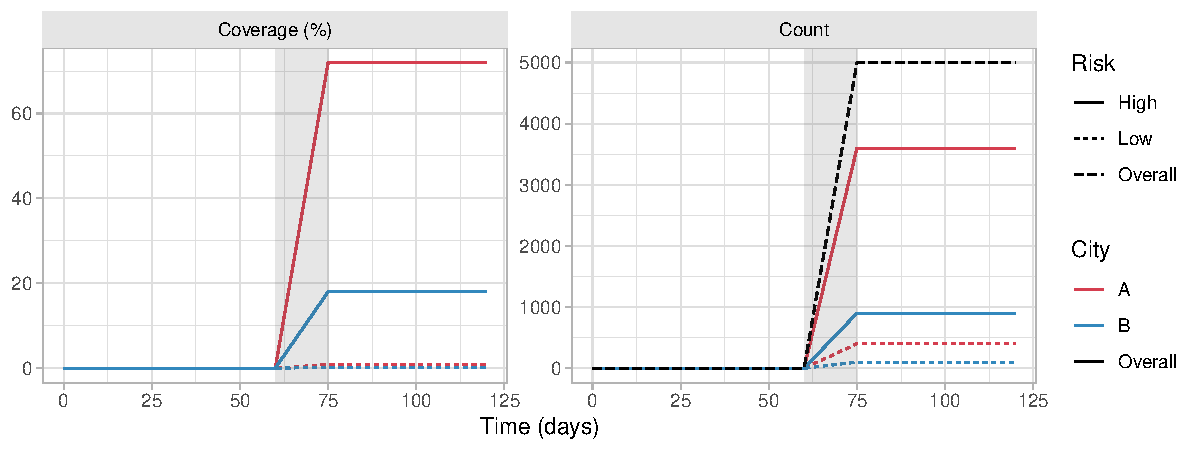
\includegraphics[width=\linewidth]{prev.vax}
  \caption{Example vaccine allocation: 80\% to city~A, and 90\% to high risk group}
  \label{fig:prev.vax}
  \floatfoot
  Gray bar indicates period of vaccine roll-out (days 60--75)
\end{figure}
\subsection{Parameterization}\label{app.model.param}
Model parameter values and stratifications are summarized in Table~\ref{tab:model.params},
repeated (verbatim) in Table~\ref{tab:model.params.app} for easier reference.
\begin{table}
  \centering
  \caption{Model parameters, including default values and ranges explored via grid sweep}
  \label{tab:model.params.app}
  \small
\begin{tabular}{llrcc}
  \toprule
  Parameter                          & Stratum                   &      Value &      Range       & Ref \\
  \midrule
  Population size                    & overall                   &    100,000 &                  & \cite{Wang2021}\tn{a} \\
                                     & fraction in city A        &        .50 &    [.20,~.80]    & \tn{a} \\
  Fraction higher risk               & city A                    &        .10 & [.01,~.50]\tn{b} & \cite{Wang2021}\tn{a} \\
                                     & city B                    &        .10 &                  & \cite{Wang2021}\tn{a} \\[1ex]
  Contact rate                       & close non-sexual, all     &          1 &                  & \tn{a} \\
                                     & sexual, low risk          &        .01 &                  & \cite{Wang2021}\tn{a} \\
                                     & sexual, high risk, city A & .178\tn{c} & [.10,~.25]\tn{b} & \cite{Wang2021,Endo2022}\tn{a} \\
                                     & sexual, high risk, city B & .178\tn{c} &                  & \cite{Wang2021,Endo2022}\tn{a} \\[1ex]
  Assortativity                      & cities, all contacts      &        .90 &    [.70,~1.0]    & \cite{Armstrong2020}\tn{a} \\
                                     & risk, close non-sexual    &          0 &                  & \tn{a} \\
                                     & risk, sexual              &        .50 &                  & \tn{a} \\
  Per-contact \SAR                   & close non-sexual          &        .05 &                  & \cite{Beer2019} \\
                                     & sexual                    &  .90\tn{c} &                  & \cite{Endo2022}\tn{a} \\[1ex]
  Initial infections                 & overall                   &         10 &                  & \tn{a} \\
                                     & fraction in city A        &        .50 &    [0.0,~1.0]    & \tn{a} \\[1ex]
  Duration of period                 & latent/incubation         &          7 &                  & \cite{Charniga2022,Thornhill2022,Miura2022} \\
                                     & infectious/symptoms       &         21 &                  & \cite{Adler2022,Thornhill2022} \\
  Fraction isolated among infected   &                           &        .50 &                  & \cite{Thornhill2022}\tn{a} \\[1ex]
  Vaccines available                 &                           &       5000 &                  & \tn{a} \\
  Vaccine effectiveness\tn{d}        &                           &        .85 &                  & \cite{Fine1988,PHAC2022vax,CDC2022vax} \\
  Vaccine prioritization sensitivity & high risk                 &        .90 &                  & \cite{TPH2022vax}\tn{a} \\
  Vaccine allocation                 & city A                    &        .50 & [0.0,~1.0]\tn{e} & --- \\
  \bottomrule
\end{tabular}
\floatfoot
All durations in days; all rates in per-day.
\SAR: secondary attack rate.
\tnt[a]{Assumed / representative.}
\tnt[b]{Calculated to fit $R_0 \in [1,2]$.}
\tnt[c]{Calculated to fit $R_0 = 1.5$,
  reflecting pre-vaccination estimate of \MPXV $R_0$ in Ontario \cite{PHO2022ont}
  via \cite{EpiNow2}.}
\tnt[d]{Leaky-type.}
\tnt[e]{Optimized parameter.}
\end{table}
\paragraph{Sexual Behaviour}
Parameterization of sexual behaviour was primarily informed by existing analyses conducted
to support mathematical modelling of \textsc{hiv}-transmission among \GBMSM in Canada
\cite[n.b. Appendix~3.2]{Wang2021}.
These analyses stratified \GBMSM into
88--94\% lower risk, with on average 4 sexual partners per-year ($\approx .01$ per day), and
6--12\% higher risk, with approximately 6-times as many partners ($\approx .07$ per day).
Our present model includes even greater partner numbers among the higher risk group (.10--.25 per day),
partly to fit \MPXV $R_0 \in [1,~2]$, and because
the 6-fold value in \cite{Wang2021} was mainly applied as a generalized proxy for
6-times higher HIV incidence.
Weighted pooling of data from three studies \cite{MaleCall2013,Lachowsky2016,Wilton2016}
suggested that approximately 12\% of respondents
reported 20+ sexual partners in the past 6 months ($\approx .11+$ per day).
Our \MPXV model also models transmission risk per-partnership,
versus per-contact (sex act) as in \cite{Wang2021};
with high \SAR, \MPXV transmission risk would be expected to be
driven more by numbers of partners than by total contacts (sex acts).
\paragraph{Monkeypox Virus (\MPXV)}
Updated epidemiological data on \MPXV infection and transmission
in the context of the present epidemic are rapidly emerging \cite{Thornhill2022,PHO2022synth}.
In the absence of high-quality evidence on
the secondary attack rate (\SAR) of sexual transmission,
we assumed a relatively high \SAR of 0.9 (per-partnership),
drawing on local patient histories, and in order to reproduce $R_0 \in [1,2]$.
We estimated $R_0 \in [1,2]$ using \MPXV case data from Ontario \cite{PHO2022ont}
before widespread vaccine roll-out (2022 May 13 -- July 4)
using the \texttt{EpiNow2} R package \cite{EpiNow2}.
\par
In another model \cite{Endo2022},
the modelled $R_0$ for a \GBMSM sexual network was greater, even for smaller \SAR.
Two main factors may explain this discrepancy in
modelled $R_0$ vs \SAR in \cite{Endo2022} vs our model.
First, isolation was not explicitly modelled in \cite{Endo2022};
thus the reported \SAR in \cite{Endo2022} can be considered as
after considering isolation, i.e., reduced.
Second, the branching process model in \cite{Endo2022}
captured greater risk heterogeneity than our model,
and focused especially on capturing the highest levels of risk (``heavy tail'').
Such heterogeneity is directly related to $R_0$
through the coefficient of variation in contact rates \cite{Anderson1986}.
Thus, this difference in model structure could further explain why
modelled $R_0$ would be greater in \cite{Endo2022}, for even similar \SAR.
Finally, our aim was to obtain generalizable insights about network-level vaccine prioritization,
rather than to model specific contexts within Ontario;
as such, we do not expect our main findings to change
with moderate changes to the model simplifications regarding transmission.
